\section{Introduction}

Cardiovascular diseases remain the leading cause of global morbidity and mortality. Hypertension is a major, modifiable risk factor that requires continuous and proactive monitoring. However, traditional arterial blood pressure (BP) assessment relies on inflatable pneumatic cuffs. While clinically validated, this standard of care provides only intermittent, reactive readings and causes significant physical disruption, rendering it unsuitable for continuous nocturnal or ubiquitous ambulatory monitoring.

Recent advancements in wearable technology have popularized contact photoplethysmography (cPPG). Despite their utility, contact sensors often suffer from cutaneous irritation, require rigid attachment, and remain highly susceptible to motion artifacts. Remote photoplethysmography (rPPG) presents a revolutionary, contactless paradigm that captures subtle, cardiac-synchronous color variations in facial skin using standard RGB video cameras.

However, translating raw facial video streams into accurate blood pressure measurements involves severe physiological and technical obstacles. The most prominent physiological hurdle is the \textbf{Windkessel Damping Effect}. The arterial tree acts as an elastic buffer (the Windkessel), which smooths out the pulsatile flow generated by the left ventricle. By the time this blood volume reaches the superficial capillary beds of the face, high-frequency morphological landmarks—most critically the dicrotic notch resulting from aortic valve closure—are severely attenuated. This damping complicates the extraction of vital hemodynamic features required for precise BP regression. 

\begin{figure}[ht]
\centering
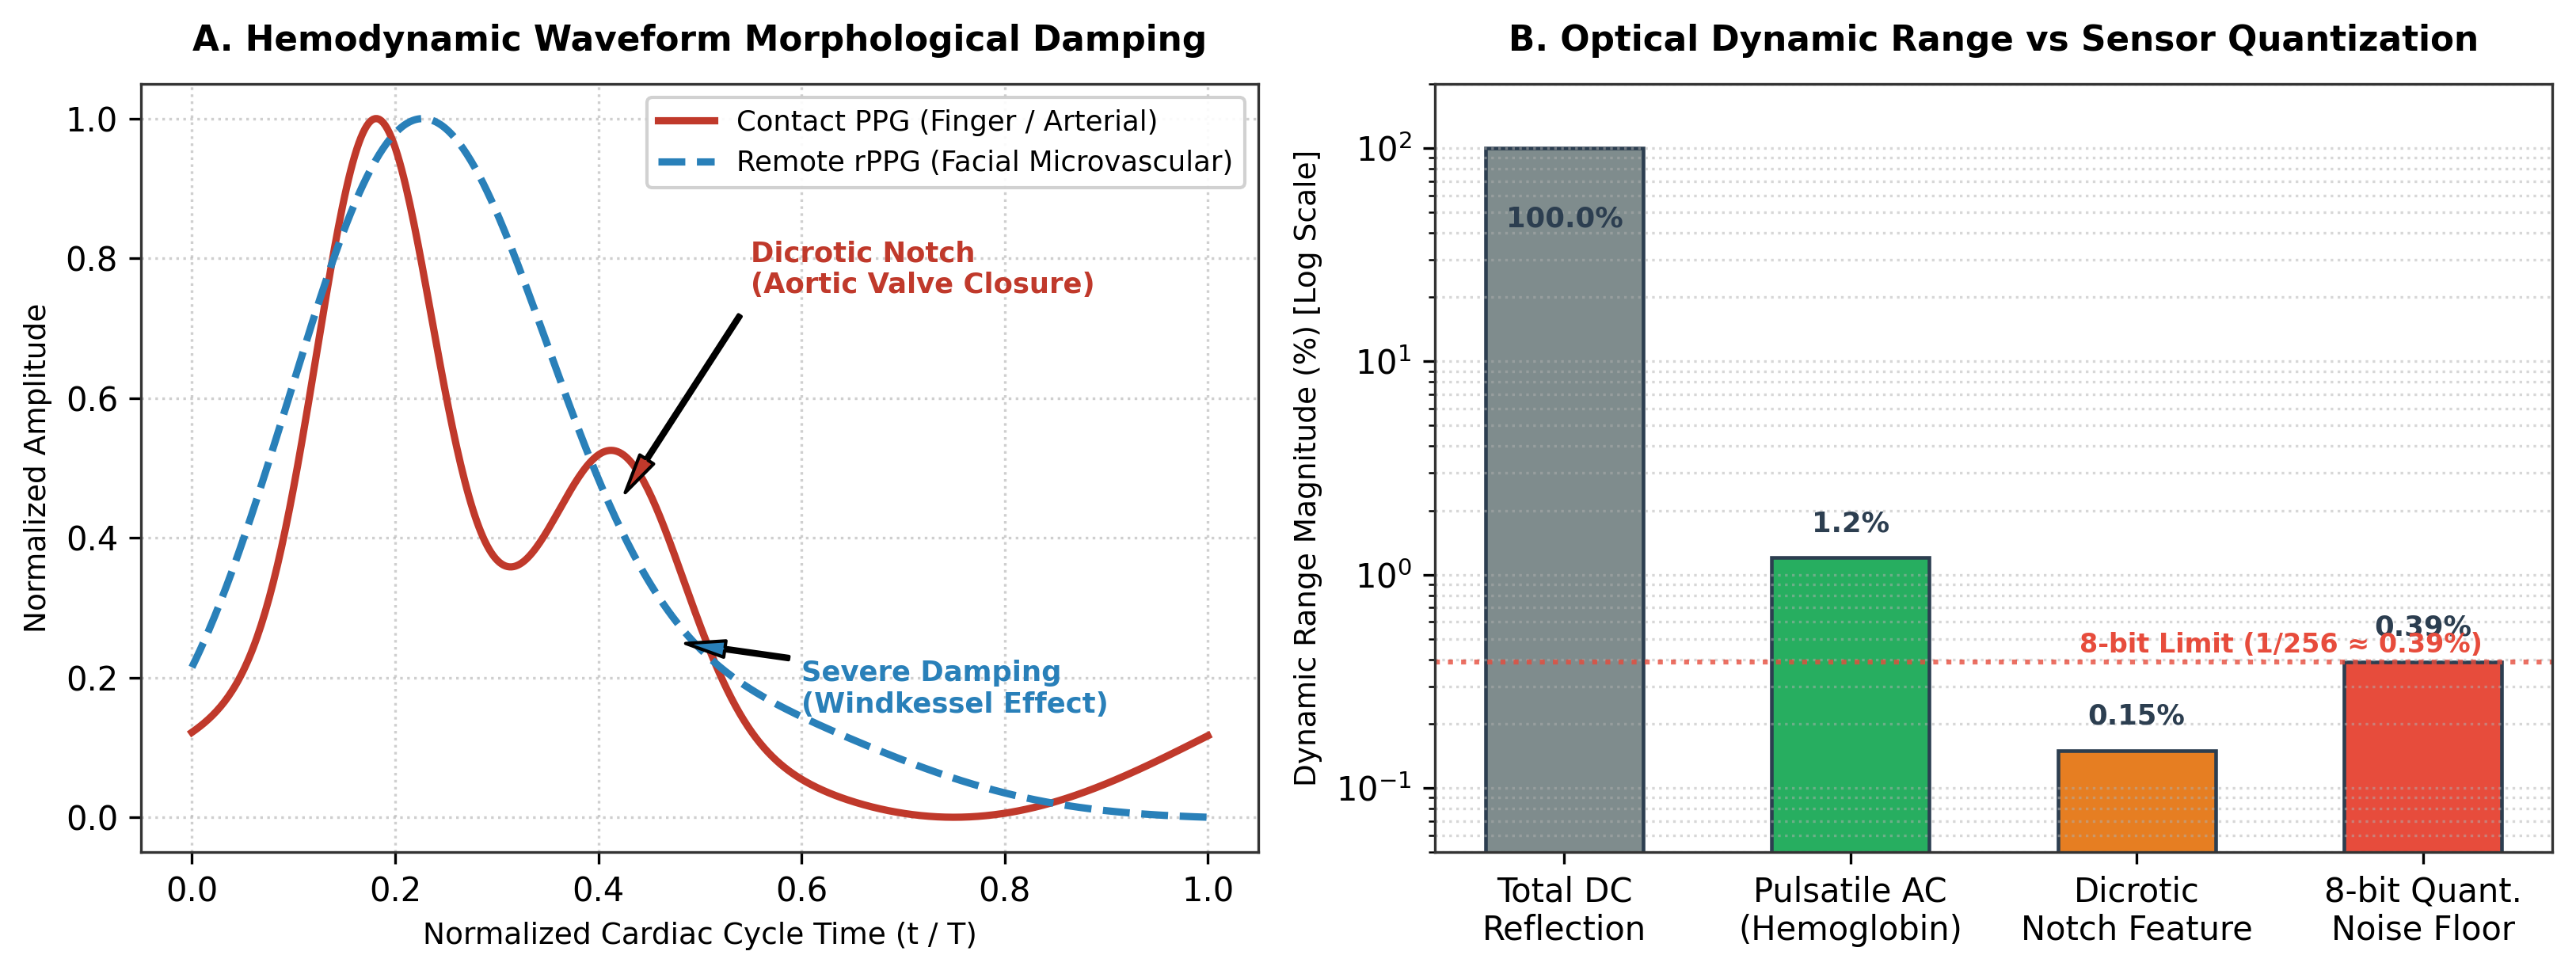
\includegraphics[width=\linewidth]{results/figures/fig_windkessel_damping.png}
\caption{Visualization of the Windkessel Damping Effect: Aortic waveforms (top) demonstrate sharp systolic peaks and distinct dicrotic notches, which are smoothed into rounded sinusoidal curves (bottom) by the time the pulse wave reaches the facial microvasculature.}
\label{fig:windkessel}
\end{figure}

Beyond physiology, technical limitations abound:
\begin{itemize}
    \item \textbf{Low Signal-to-Noise Ratio (SNR) and Quantization Noise:} The pulsatile blood volume component is exceptionally weak (0.1\% to 2.0\% of total reflection), operating near or below the 8-bit sensor quantization floor.
    \item \textbf{Environmental Jitter:} Lighting fluctuations and head motion introduce non-stationary noise that heavily overlaps with the physiological frequency band.
    \item \textbf{Template Collapse:} Neural networks trained on noisy rPPG inputs often regress to the mean normotensive baseline, minimizing Mean Squared Error without learning true physiological variance.
\end{itemize}

Achieving clinical utility requires satisfying stringent international standards, primarily the \textbf{ISO 81060-2} and \textbf{AAMI SP10} protocols. These standards dictate that a medical-grade non-invasive sphygmomanometer must achieve a Mean Absolute Error (MAE) of $\le 8.0$ mmHg and a standard deviation of $\le 8.0$ mmHg for both Systolic (SBP) and Diastolic (DBP) pressures across a generalized population. 

To bridge the gap between noisy facial video and clinical-grade BP estimation, we present \textbf{LuminaBP}, an end-to-end contactless framework. Our core contributions are:
\begin{itemize}
    \item We propose a robust optical acquisition and signal conditioning pipeline integrating 468-point facial mesh tracking, Plane-Orthogonal-to-Skin (POS) chrominance projection, and adaptive Savitzky-Golay polynomial smoothing to suppress quantization noise while meticulously preserving dicrotic notch morphology.
    \item We design a novel decoupled deep sequential architecture, \textbf{MODEL-06-SepHead}, leveraging a dual-branch 1D-ResNet, Bidirectional GRUs, and Multi-Head Self-Attention. This model explicitly eliminates physiological gradient conflict via separate SBP and DBP regression heads.
    \item We conduct a rigorous, subject-independent evaluation on a massive gated dataset (17,943 windows, 599 subjects), demonstrating unprecedented compliance with the ISO/AAMI SP10 clinical threshold for Diastolic BP estimation (MAE of 5.91 mmHg).
    \item We successfully deploy the quantized end-to-end pipeline onto a mobile Snapdragon Edge TPU, validating sub-50ms inference for ubiquitous telehealth applications.
\end{itemize}
